%!TEX root = ../thesis.tex

\section{背景}
移動ロボットにおけるナビゲーションは,目的地までロボットを誘導する制御技術として広く利用されており,物流や農業,製造業などで活用されている.
一般的には LiDAR や IMU ,ホイールエンコーダなど複数のセンサから得られるデータと占有格子地図などのメトリックマップを使用することでロボットを目的地まで制御する.
一方で,後述するようにカメラ画像と深層学習に基づくナビゲーション技術の研究も進んでいる.

Felipe ら\cite{codevilla2018endtoend}は視覚を入力とした end-to-end 学習により自動運転を行う手法において,右折や左折といった行動をネットワークの入力に加えることで,性能が向上することを報告している.
本研究室の岡田ら\cite{okada2020}\cite{okada2021}は,\figref{fig:imitation_sys}にように,メトリックマップに基づく経路追従行動を視覚を入力として模倣学習することで,視覚に基づて経路追従するシステムを提案した.
この手法では,センサとメトリックマップを入力としたルールベース制御器によって生成されたヨー方向の角速度とロボットに取り付けたカメラから取得した RGB 画像をペアにしてデータセットに加えて学習する.
学習後はカメラ画像のみを用いて,学習した経路を追従できることが確認されている.
% この手法では,センサとメトリックマップを入力とした ROS の navigation パッケージによって生成されたナビゲーションの角速度とカメラ画像をペアにして学習し,学習後はカメラ画像のみを用いて経路追従行動できることが確認されている.
% この手法では,一般的な模倣学習が人間のステアリング操作を模倣するのに対し,ナビゲーションシステム自体の行動を模倣する点で特徴的であり,データセットの収集を自動で行うことができる.
% これらの技術の有効性は,シミュレーションおよび実ロボットの実験により検証されており,視覚に基づくナビゲーションで一定の経路追従性能を達成できることが確認されている.
\begin{figure}[h]
     \centering
     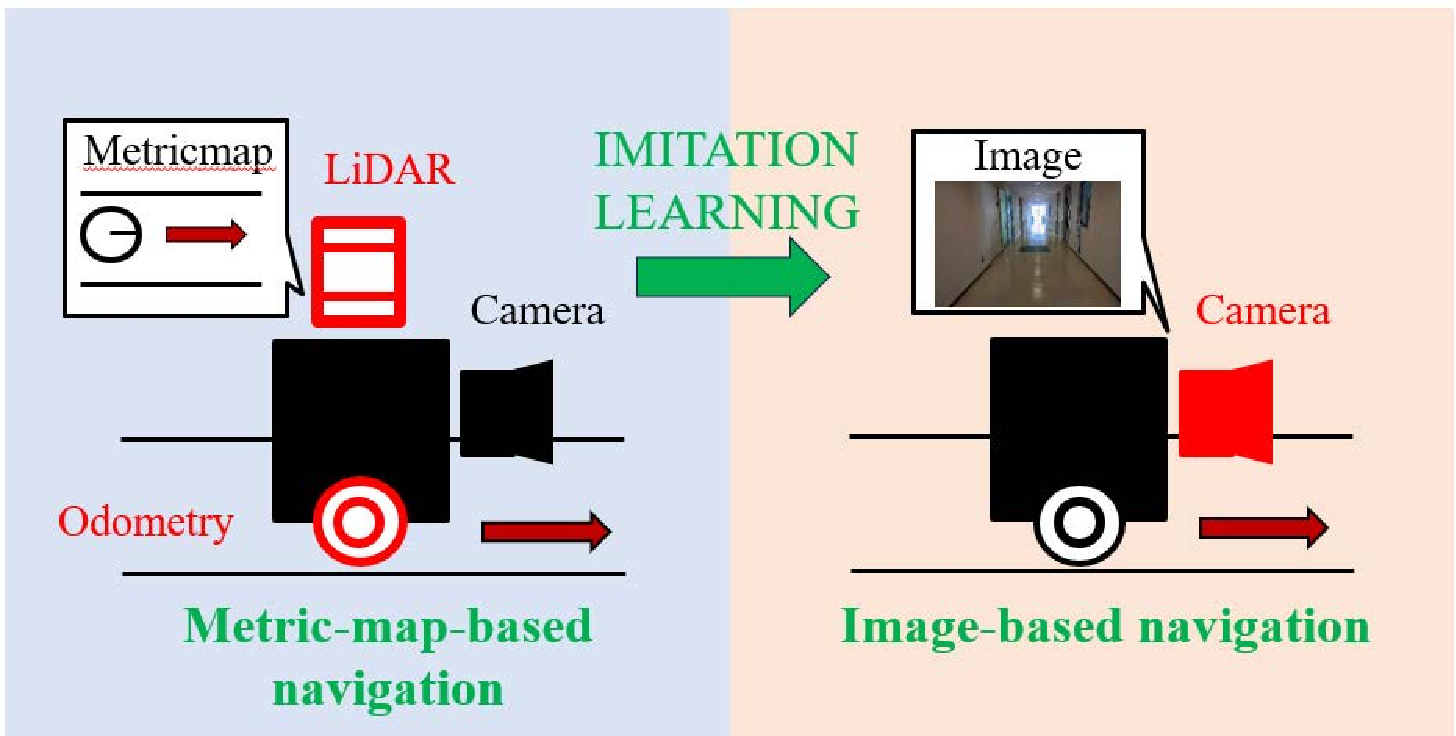
\includegraphics[width=120mm]{images/pdf/ishiguro/system.pdf}
     \caption{Imitation method of path-tracking behavior}
     \label{fig:imitation_sys}
\end{figure}

また,春山ら\cite{haruyama2023}はカメラ画像とシナリオに基づいて,任意の目的地まで経路追従するシステムを提案している.
ここでのシナリオとは島田ら\cite{shimada2020}が提案した,「条件」と「行動」に関する単語を組みわせて構成する文章を指す.
春山らの手法では,岡田らの視覚に基づいたナビゲーションに加え,カメラ画像から通路の種類を分類,シナリオによって目標方向を決定し,経路を選択する機能を追加している.
春山らの先行研究では,島田らが提案した 50 例のシナリオの中から 7 例を選定し,そのすべてで経路追従が可能であることを確認している.

春山らの先行研究では,島田らが作成したシナリオの中で,以下\figref{fig:cit3f}の青枠で示すエリアを対象としたシナリオを用いている.
このエリアはホワイエと呼ばれるスペースを一部を含むものの,壁や床の色が類似しており,一貫性のある環境といえる.
一方で\figref{fig:cit3f}の赤色で示すエリアを含むシナリオでは,地面の色が異なるエリアやホワイエを含んでおり,視覚に基づいて経路追従するのがより困難な環境と考えられる.
また,春山らの先行研究では対象としたシナリオすべてで目的地まで到達できることが確認されており,失敗の要因は判明していない.
失敗する場合は要因を調査することで,システムの改良点について考察できるようになる.

また,カメラ画像と深層学習に基づくナビゲーションの先行研究では,Felipeらが目標方向ごとにモデルを切り替えるネットワークが経路追従の成功率を高められると報告している.
提案されたネットワークを使用することで,春山らが使用していたネットワークより経路追従の成功率を向上させることができる可能性がある.

\begin{figure}[htbp]
     \centering
     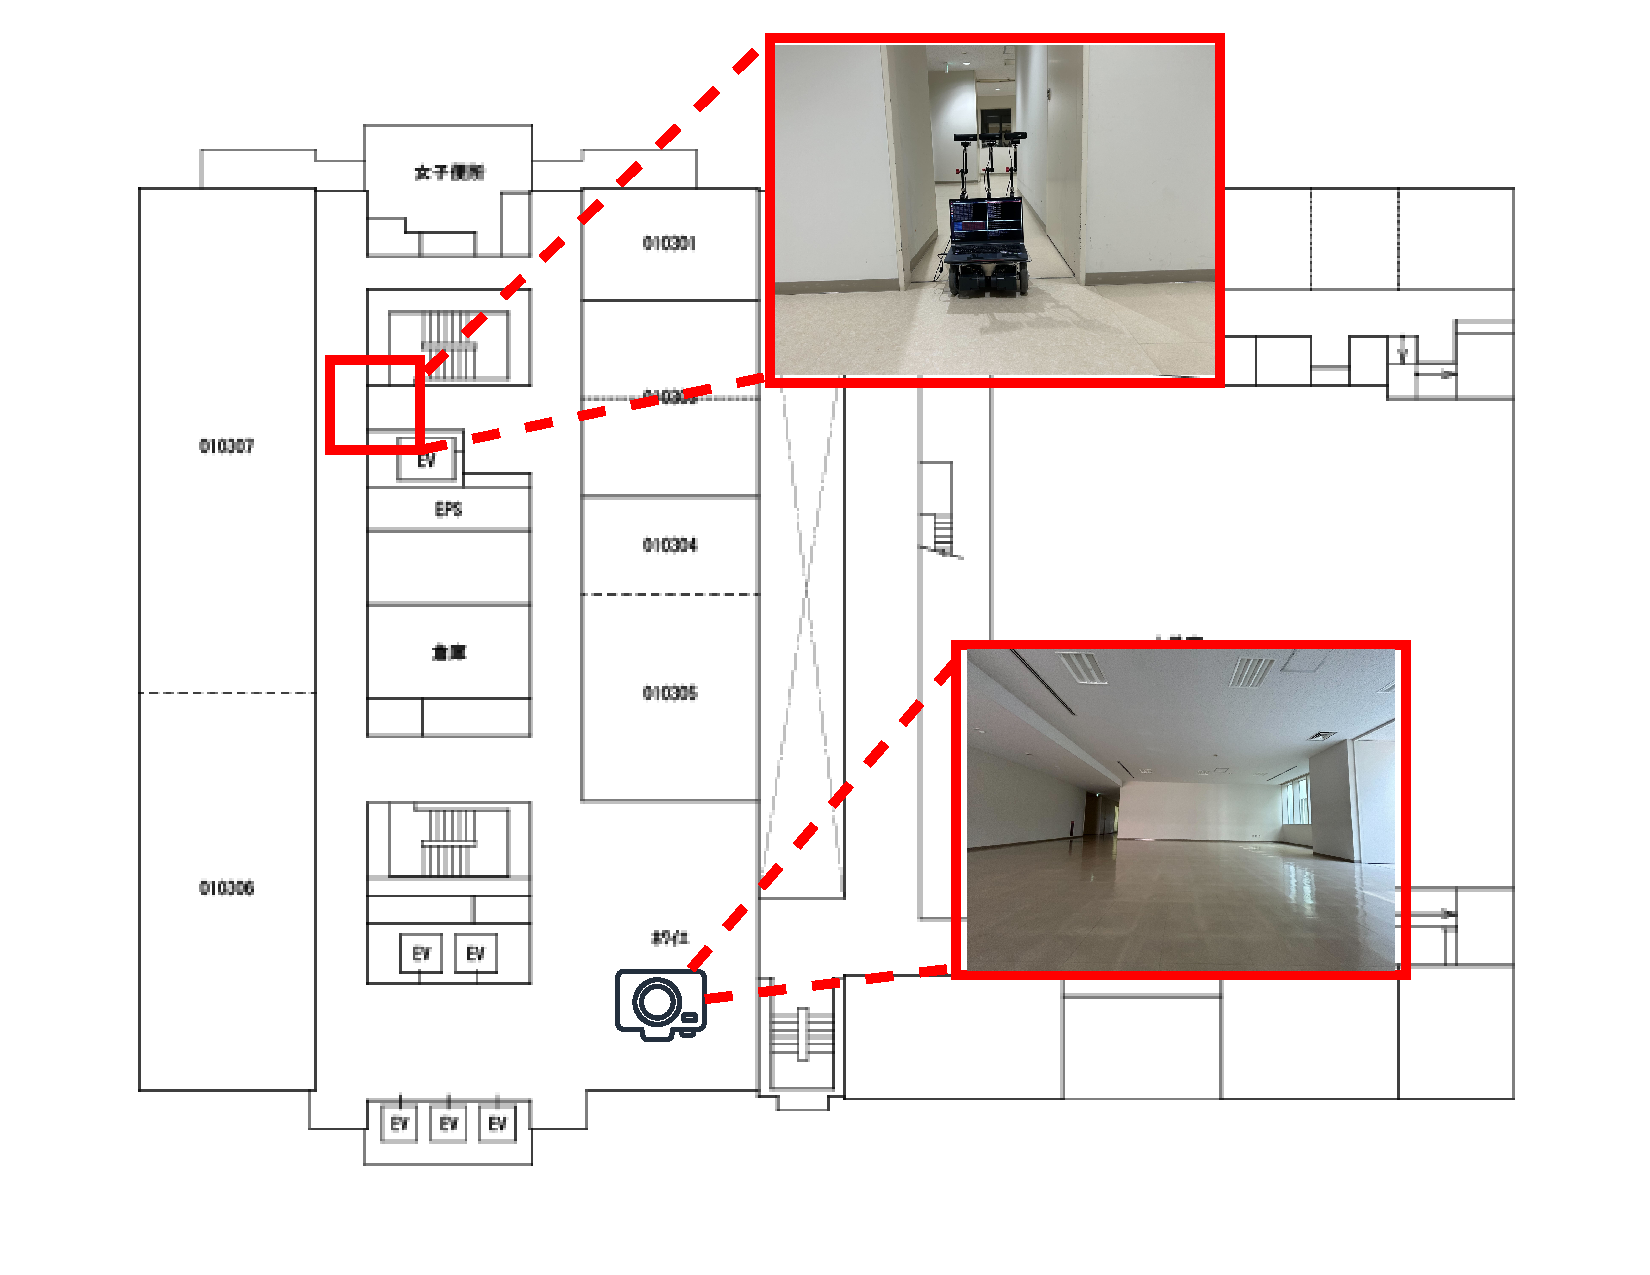
\includegraphics[width=130mm]{images/pdf/ishiguro/cit3f.pdf}
     \caption{Experimental environment}
     \label{fig:cit3f}
\end{figure}

\newpage
